\documentclass[btech,thesis,twoside]{iist}
\usepackage{times} % Or your specific thesis class
\usepackage{amsmath}
\usepackage{amsfonts} % For mathbb if needed
\usepackage{amssymb}  % For math symbols
\usepackage{bm}       % For bold math symbols if preferred (e.g., \bm{A})
\usepackage{amsmath}
\usepackage{amsfonts}
\usepackage{amssymb}
\usepackage{bm}
\usepackage{graphicx} % Added for potential figure reference
\usepackage{algorithm}
\usepackage{algorithmicx}
\usepackage{amsmath}
\usepackage{amssymb}
\usepackage{graphicx} % For including figures
\usepackage{booktabs} % For professional-looking tables (optional, but recommended)
\usepackage{multirow} % For tables with multi-row cells (optional)
\usepackage{subcaption} % For subfigures (optional)
\usepackage{algpseudocode}
% Add hyperref if you want clickable refs to equations/sections
\usepackage{hyperref}
% Add hyperref if you want clickable refs
% \usepackage{hyperref}
% \hypersetup{colorlinks=true, linkcolor=blue, citecolor=green, urlcolor=cyan}

% Define figure/table reference commands if needed
\newcommand{\reffig}[1]{Figure~\ref{#1}}
\newcommand{\reftab}[1]{Table~\ref{#1}}
\newcommand{\refsec}[1]{Section~\ref{#1}}
\hypersetup{colorlinks=true, linkcolor=blue, citecolor=green, urlcolor=cyan}
\title{Decentralized Multi-Agent Path Planning }
\author{Velamala Rahul}
\studentid{SC21B127}
\advisor{Dr.Sourav Bhowmick}
\specialization{Electronics and Communication Engineering (Avionics)}
\department{Avionics}
\date{May 2025}


%% ---- Document starts here ---- %%
\begin{document}

%% ---- Make the initial set of pages ---- %%
\maketitle % Title page
\makecertificate % Certificate 
\makedeclaration % Declaration
 % Dedication
\makeacknowledgements % Acknowledgements
\makeabstract % Abstract
\maketableofcontents % Table of contents
\makelistoffigures % List of figures
% \makelistoftables % List of tables
%\makelistofalgorithms % List of algorithms
\makeabbreviations % List of abbreviations
% \makenomenclature % Nomenclature (for symbols used)

% Initialize chapter settings; DO NOT comment this line
\makechaptersettings 


%% ---- Start chapters here ---- %%
%======================================
% CHAPTER 1: INTRODUCTION
% ==================================================
\chapter{Introduction}
\label{chap:introduction}
\section{Motivation}
Multi-robot systems are increasingly common in a variety of applications, from automated warehousing and logistics \cite{Wurman2008} to environmental monitoring, search and rescue, surveillance, and planetary exploration \cite{Parker2008}. 
Coordinating multiple robots to navigate complex, shared environments while avoiding collisions is a fundamental challenge for the success of these systems.The Multi-Robot Path Planning (MRPP), or Multi-Agent Path Finding (MAPF) \cite{Stern2019MAPFSurvey} problem addresses this core requirement of computing collision-free paths for a group of robots from their initial locations to target goal points.

Although centralized methods for MRPP may be able to provide optimal solutions \cite{Sharon2015CBS}, they assume global knowledge and a coordinator node, resulting in strong computational bottlenecks and scalability problems as the size of the team increases \cite{Standley2011Complete}. In addition, most real-world situations naturally create decentralized constraints. Robots can be deployed with bounded sensing ranges, limited peer-to-peer communication capacity, and no access to global positioning systems or a stable central controller \cite{Li2021GNNCoordination, VanDenBerg2008ORCA}. Under such decentralized environments, each robot needs to make navigation decisions based only on its local observations and information it receives from neighboring teammates. This requires efficient strategies for information exchange and distributed coordination to realize shared objectives.

Recent advancements have been looking into learning-based methods using Graph Neural Networks (GNNs),Reinforcement Learning to formulate decentralized MRPP policies \cite{Li2021GNNCoordination, Tolstay2020LearningDecentralized}. GNNs are well-adapted to representing the communication and relational structure present in multi-robot teams. A prominent framework proposed by Li et al. \cite{Li2021GNNCoordination} uses a Convolutional Neural Network (CNN) for feature extraction from local observations and a GNN to enable inter-robot communication and coordinate action. 

\section{Problem Statement}
\label{sec:problem_statement}

This thesis addresses the problem of decentralized Multi-Robot Path Planning (MRPP) in environments where robots have limited capabilities. We consider scenarios where:
\begin{itemize}
    \item Robots operate in a shared environment with static obstacles.
    \item Each robot possesses only local sensing capabilities, perceiving its surroundings within a limited Field-of-View (FOV).
    \item Robots lack access to global information, such as a complete map or absolute positioning .
    \item Communication is restricted to peer-to-peer interactions within a predefined communication radius ($r_{comm}$). Robots can only exchange information directly with neighbors within this range.
    \item The goal is for all robots to navigate from their individual start locations to their respective goal locations efficiently avoiding collisions with obstacles and other robots.
\end{itemize}

Although GNN-based methods such as Li et al. \cite{Li2021GNNCoordination} provide a framework for learning decentralized coordination, the limitation arises from their dependence on a \textbf{fixed, predefined communication range}, typically implemented as K-hop message passing. In this approach, each robot aggregates information only from peers within a fixed number of communication hops (K). This fixed structure presents the drawback that the optimal extent of information sharing may vary depending on factors such as environmental complexity, the number of robots, the density of local robots and the specific situation encountered during navigation. A single manually tuned value of K is unlikely to be optimal for all these diverse conditions. Selecting the best K often requires extensive empirical tuning or heuristics, limiting the adaptability and potentially the peak performance of the learned coordination policy. This inflexibility motivates the need for a communication mechanism that can dynamically adapt the extent of information propagation or learn the most suitable range from the data.

\newpage
\section{Objectives}
\label{sec:objectives}

The primary goal of this thesis is to enhance decentralized MRPP by incorporating adaptive communication, addressing the limitations of fixed interaction ranges in prior GNN-based work \cite{Li2021GNNCoordination}. The specific objectives are:

\subsection{Task 1: Integrate Adaptive Communication Mechanism}
\label{subsec:obj_integrate}
Replace the fixed K-hop GNN communication module \cite{Li2021GNNCoordination} with Adaptive Diffusion Convolution (ADC) \cite{Zhao2021ADC}. This aims to enable the network to automatically learn the optimal information diffusion extent ($t$) during training, adapting the communication neighborhood based on the task.

\subsection{Task 2: Analyze Theoretical Properties}
\label{subsec:obj_analysis}
Briefly analyze and contrast the theoretical stability and spectral filtering properties of the ADC layer relative to standard fixed-K GCN layers \cite{Kipf2017GCN}, highlighting potential advantages in stability \cite{Zhao2021ADC, Gama2019StabilityGNN} and adaptive filtering.

\subsection{Task 3: Empirically Evaluate Performance}
\label{subsec:obj_evaluation}
Quantitatively evaluate the proposed ADC-enhanced MRPP framework using imitation learning on expert (CBS \cite{Sharon2015CBS}) demonstrations. Performance will be measured by Success Rate (SR) and Convergence Time (CT) in simulated grid environments and compared against fixed-K GNN baselines.

\subsection{Task 4: Assess Adaptivity and Generalization}
\label{subsec:obj_adaptivity}
Investigate the practical benefits of adaptivity by comparing performance across varying environmental conditions (e.g., obstacle densities). Assess the generalization capabilities of the ADC model versus fixed-K models when tested on conditions different from training, supported by relevant ablation studies.

\newpage

\section{Contributions}
\label{sec:contributions}

The primary contributions of this thesis are:
\begin{itemize}
    \item Integration of Adaptive Diffusion Convolution (ADC) \cite{Zhao2021ADC} into a decentralized MRPP framework \cite{Li2021GNNCoordination}, enabling the automatic learning of adaptive communication ranges ($t$) instead of relying on fixed K-hops.
    \item Theoretical analysis highlighting improved stability properties of the ADC layer compared to standard GCN layers within the MRPP context.
    \item Empirical demonstration, via simulation and imitation learning, that the ADC-enhanced framework achieves superior success rates compared to fixed-K GNN baselines across various environments.
    \item Evidence showing the ADC approach offers better adaptability to different environmental conditions (e.g., obstacle densities) and improved generalization to unseen scenarios compared to fixed-range methods.
\end{itemize}

\section{Report Organization}
\label{sec:report_organization}

The remainder of this thesis is structured as follows:

\begin{itemize}
    \item \textbf{\hyperref[chap:literature_review]{Chapter 2 (Literature Review)}:} Provides a comprehensive review of existing work in Multi-Robot Path Planning, covering centralized, decentralized, and learning-based approaches, with a focus on GNN-based methods and adaptive graph techniques.

    \item \textbf{\hyperref[chap:background]{Chapter 3 (Background and Theoretical Foundations)}:} Introduces the necessary theoretical background on graph theory, Graph Neural Networks (GNNs), graph signal processing, graph diffusion processes, and the Adaptive Diffusion Convolution (ADC) mechanism.

    \item \textbf{\hyperref[chap:dataset]{Chapter 4 (Dataset Generation and Preprocessing)}:} Details the process of generating the synthetic MRPP datasets used for training and evaluation, including the simulation environment setup, expert planner (CBS) usage, data representation, and preprocessing steps.

    \item \textbf{\hyperref[chap:methodology]{Chapter 5 (Framework \& Methodology)}:} Describes the architecture of the proposed ADC-enhanced MRPP framework in detail, explaining the CNN encoder, the ADC communication module, the MLP action selector, and the imitation learning training setup.

    \item \textbf{\hyperref[chap:results]{Chapter 6 (Results)}:} Outlines the experimental methodology, including implementation details, evaluation metrics, baseline models, and presents the quantitative and qualitative results comparing the proposed ADC approach with fixed-K GNN baselines, including ablation and generalization studies.

    \item \textbf{\hyperref[chap:conclusion]{Chapter 7 (Conclusion \& Future Work)}:} Interprets the key experimental results, discusses the implications and limitations of the study, summarizes the main findings and contributions, and suggests potential directions for future research.
\end{itemize}
% Add bibliography command here in your main file: \bibliography{your_bib_file}

\chapter{Literature Review}
\label{chap:literature_review}
\section{Overview of Decentralized Multi-Agent Path Planning}
This chapter presents a comprehensive review of the methods and frameworks used in modern multi-agent path planning (MAPF) systems, especially those based on decentralized architectures.
It investigates various approaches to path planning in multi-robot systems, highlights the evolution towards decentralized and dynamically adaptive strategies, and discusses the increasing relevance of decentralized MAPF in complex and uncertain environments. Each section explores key concepts, technological advancements, and inherent challenges in developing and implementing decentralized MAPF solutions. The chapter aims to outline the state of the art, emphasizing practical challenges and theoretical complexities that define this research field.

\section{Multi-Agent Path Planning System Architectures}
A multi-agent path planning system can be broadly categorized based on its architecture, which dictates information flow and decision-making processes:
\begin{itemize}
    \item \textbf{Centralized Architectures:} In centralized systems, a single planning unit possesses complete knowledge of all agents, their goals, and the environment. This unit computes paths for all agents, ensuring coordination and often aiming for global optimality. Algorithms such as M* and CBS are key examples of this approach.
    \item \textbf{Decentralized Architectures:} Decentralized systems distribute planning and decision-making among individual agents. Each agent plans its path based on local information and limited communication with neighbors. Methods like VO and ORCA are representative of decentralized strategies.
    \item \textbf{Coupled Approaches:} Coupled approaches, often found in centralized systems, consider the joint state space of all agents simultaneously. This allows for optimal solutions but suffers from scalability issues. CBS and M* are examples of coupled approaches.
    \item \textbf{Decoupled Approaches:} Decoupled approaches simplify planning by considering each agent's path individually, addressing conflicts reactively. VO and ORCA are examples of decoupled methods that prioritize computational efficiency.
    \item \textbf{Networked Topologies:} Multi-agent systems often operate within networked topologies, where communication and coordination are constrained by the network structure. Graph-based representations, like those used in GNNs and algorithms like PRIMAL, are well-suited to model and exploit these topologies for decentralized MAPF.
\end{itemize}

\section{Centralized Multi-Agent Path Planning Techniques}
Centralized MAPF approaches, while offering optimality guarantees under certain conditions, face scalability limitations and single points of failure. This section reviews key centralized techniques and their characteristics.

\subsection{Optimal Centralized Algorithms: M* and ICTS}
Optimal centralized algorithms like M* \cite{Standley2011Complete} % Corrected citation key if needed
and ICTS (Increasing Cost Tree Search) aim to find solutions with the minimum total cost (e.g., sum of path lengths) for all agents. M* guarantees optimality and completeness by systematically exploring the joint state space of all agents. ICTS, while also striving for optimality, improves efficiency over basic search algorithms by focusing on conflict resolution within a tree-based search framework. However, the computational complexity of these algorithms grows exponentially with the number of agents and environment size, limiting their applicability to large-scale problems.

\subsection{Conflict-Based Search (CBS)}
Conflict-Based Search (CBS) \cite{Sharon2015CBS} % Corrected citation key if needed
is a prominent centralized MAPF algorithm that efficiently finds optimal or near-optimal solutions by iteratively resolving conflicts between agents paths. CBS operates on a two-level search structure: a high-level search that identifies and resolves conflicts by adding constraints, and a low-level search (typically A*) that replans paths for individual agents under these constraints. CBS significantly improves scalability compared to brute-force search methods but still faces computational challenges with increasing agent density and complex environments. Despite its efficiency improvements over purely exhaustive searches, CBS remains computationally expensive for very large teams or highly complex environments.

\section{Decentralized Multi-Agent Path Planning Techniques}
Decentralized MAPF methods prioritize scalability and robustness by distributing planning and decision-making among individual agents. This section reviews key decentralized approaches, including velocity obstacle based methods and learning-based techniques.

\subsection{Velocity Obstacle (VO) and Optimal Reciprocal Collision Avoidance (ORCA)}
Velocity Obstacle (VO) \cite{VanDenBerg2008ORCA} % Corrected citation key if needed
and its refinement, Optimal Reciprocal Collision Avoidance (ORCA), are classic decentralized approaches for collision avoidance. VO defines a velocity obstacle for each agent based on the relative velocities and positions of neighboring agents. ORCA improves upon VO by ensuring reciprocal collision avoidance and smoother trajectories. These methods are computationally efficient and reactive, enabling real-time collision avoidance in dynamic environments. However, VO and ORCA are primarily reactive and may not guarantee goal achievement or optimality in complex scenarios, and can sometimes lead to local minima or deadlocks in tightly constrained spaces.

\subsection{Decentralized Planning with Graph Neural Networks (GNNs) and PRIMAL }
Recent advancements explore learning-based decentralized MAPF, particularly utilizing Graph Neural Networks (GNNs) and Reinforcement Learning (RL). GNNs, as demonstrated by Li et al. \cite{Li2021GNNCoordination}, % Corrected citation key if needed
are well-suited for decentralized MAPF due to their ability to model agent interactions within a graph structure, facilitating distributed information aggregation and decision-making. However, standard GNN approaches often rely on aggregating information from a fixed K-hop neighborhood, which may not be optimal across diverse situations. PRIMAL (Pathfinding via Reinforcement and Imitation Multi-Agent Learning) \cite{Sartoretti_et_al_2019} combines imitation learning from expert demonstrations with reinforcement learning to train decentralized policies, often without explicit communication modeling.

To address the limitations of fixed communication ranges in GNNs, adaptive graph methods like Adaptive Diffusion Convolution (ADC) \cite{Zhao2021ADC} have been proposed. ADC replaces discrete K-hop aggregation with a learnable diffusion process, allowing the network to automatically determine the appropriate extent of information propagation based on the task and data. Integrating such adaptive diffusion mechanisms into GNNs for MAPF holds the potential to improve coordination policies by dynamically adjusting the communication neighborhood size, enhancing adaptability compared to fixed-K approaches. These learning-based methods, especially those incorporating adaptive communication, are promising for achieving more sophisticated and adaptable coordination in decentralized systems.

\section{Relevance of Decentralized Multi-Agent Path Planning Systems}
Decentralized MAPF systems are increasingly relevant due to their inherent advantages in various robotic applications:
\begin{itemize}
    \item \textbf{Scalability:} Decentralized approaches scale more effectively to large teams of robots, as computational load is distributed across agents rather than concentrated in a central unit.
    \item \textbf{Robustness and Fault Tolerance:} Decentralized systems are more robust to failures, as the system can continue operating even if individual agents or communication links fail.
    \item \textbf{Adaptability to Dynamic Environments:} Decentralized agents can react more quickly to changes in the environment, as they rely on local sensing and communication rather than waiting for global updates.
    \item \textbf{Real-time Performance:} Decentralized algorithms are often more computationally efficient, enabling real-time path planning and execution, crucial for dynamic applications.
    \item \textbf{Versatility and Flexibility:} Decentralized systems can be deployed in diverse environments, including those with limited communication infrastructure or unknown topologies.
    \item \textbf{Cost-Effectiveness:} Decentralized systems can reduce reliance on expensive centralized computing and communication infrastructure, potentially lowering overall system costs.
    \item \textbf{Applications in Complex Domains:} Decentralized MAPF is essential for applications in domains like warehouse automation, autonomous driving, search and rescue, and space exploration, where large teams of robots must operate autonomously in dynamic and uncertain conditions.
\end{itemize}

\section{Challenges in Decentralized MAPF}
Despite their advantages, Decentralized MAPF systems face several significant challenges:
\begin{itemize}
    \item \textbf{Sub-optimality:} Decentralized solutions may not guarantee global optimality, as agents make decisions based on limited local information.
    \item \textbf{Deadlocks and Local Minima:} Insufficient coordination in decentralized systems can lead to deadlocks or agents becoming trapped in local minima.
    \item \textbf{Partial Observability:} Agents typically have only partial views of the environment, making it difficult to plan globally optimal paths and anticipate the actions of distant agents.
    \item \textbf{Communication Constraints:} Limited communication range, bandwidth, or reliability can hinder effective coordination in decentralized systems. Determining the optimal range and information to share is also a challenge.
    \item \textbf{Dynamic and Uncertain Environments:} Adapting to dynamic obstacles, changing goals, and noisy sensor data in real-time remains a significant challenge for decentralized MAPF.
    \item \textbf{Coordination Complexity:} Designing effective coordination mechanisms in decentralized systems, especially for complex tasks and dense agent populations, is non-trivial.
    \item \textbf{Verification and Validation:} Verifying the correctness and safety of decentralized MAPF algorithms, particularly in safety-critical applications, can be challenging.
    \item \textbf{Adaptability and Learning in Decentralized Settings:} Enabling decentralized agents to learn and adapt to new environments and tasks autonomously, especially concerning communication strategies, is an ongoing research area.
    \item \textbf{Balancing Reactivity and Proactiveness:} Decentralized agents need to be reactive to local changes while also exhibiting proactive behavior to achieve long-term goals and avoid potential future conflicts.
    \item \textbf{Ensuring Fairness and Efficiency:} In multi-agent systems, ensuring fairness in resource allocation and efficient overall system performance requires careful design of decentralized algorithms.
\end{itemize}

\section{Chapter Summary}
This chapter has provided a literature review focusing on Decentralized Multi-Agent Path Planning. We have explored the spectrum of MAPF approaches, from centralized optimal algorithms like M* and CBS to decentralized reactive methods like VO and ORCA, and emerging learning-based techniques utilizing GNNs and RL like PRIMAL. A key challenge identified in learning-based methods is the reliance on fixed communication ranges. The chapter highlighted the relevance and advantages of decentralized MAPF in complex robotic applications, while also outlining the significant challenges that remain in achieving robust, efficient, and truly autonomous multi-robot systems. In subsequent chapters, we will delve into our proposed decentralized path planning framework, addressing some of these challenges by leveraging Adaptive Diffusion Convolution (ADC) to enhance coordination and adaptability by learning effective communication ranges. We aim to contribute to the field by exploring how adaptive communication mechanisms can improve the performance and robustness of decentralized MAPF systems.
% ============================================================
% CHAPTER 3: BACKGROUND AND THEORETICAL FOUNDATIONS
% ============================================================
\chapter{Background and Theoretical Foundations}
\label{chap:background}

This chapter lays the groundwork for understanding the proposed decentralized multi-robot path planning framework enhanced with Adaptive Diffusion Convolution (ADC). We begin by introducing fundamental concepts from graph theory, which provide the mathematical language for representing multi-robot systems and their interactions. We then delve into Graph Neural Networks (GNNs), explaining their general architecture and how they process graph-structured data, highlighting the limitations of standard fixed-neighborhood approaches. Subsequently, we explore concepts from graph signal processing and graph diffusion processes, focusing on the graph heat kernel, which forms the basis for ADC. Finally, we detail the Adaptive Diffusion Convolution mechanism itself, explaining how it enables learnable, adaptive information propagation on graphs.

\section{Graph Theory Essentials}
\label{sec:graph_theory}

Graphs provide a natural and powerful way to model the relationships and interactions within multi-robot systems.

A \textbf{graph} is formally defined as a pair $G = (V, E)$, where $V$ is the set of vertices (or nodes) and $E \subseteq V \times V$ is the set of edges connecting pairs of vertices. In the context of MRPP, the set of robots typically constitutes the vertex set $V = \{1, ..., N\}$, where $N$ is the total number of robots.

An \textbf{edge} $(i, j) \in E$ signifies a relationship or potential interaction between robot $i$ and robot $j$. In decentralized MRPP, edges often represent the possibility of direct communication or sensing between robots. If the relationship is symmetric (i.e., if robot $i$ can communicate with $j$, then $j$ can communicate with $i$), the graph is \textbf{undirected}. If the relationship has a direction, the graph is \textbf{directed}. In many MRPP scenarios, communication links are bidirectional, leading to undirected graphs.

The structure of the graph, particularly the communication links, can change over time as robots move. Therefore, we often consider a \textbf{time-varying graph} $G_t = (V, E_t)$ at each discrete time step $t$. An edge $(i, j) \in E_t$ might exist if the distance between robots $i$ and $j$ at time $t$, denoted by $\|p_i(t) - p_j(t)\|$, is less than or equal to a predefined communication radius $r_{comm}$.

The structure of a graph $G_t$ at time $t$ is commonly represented using matrices:

\begin{itemize}
    \item \textbf{Adjacency Matrix ($A_t$):} An $N \times N$ matrix where $[A_t]_{ij} = 1$ if $(i, j) \in E_t$ and $i \neq j$, and $[A_t]_{ij} = 0$ otherwise. For undirected graphs, $A_t$ is symmetric ($A_t = A_t^T$). Often, self-loops are added, resulting in $\hat{A}_t = A_t + I$, where $I$ is the identity matrix. This allows a node to consider its own features during aggregation.
    \item \textbf{Degree Matrix ($D_t$):} An $N \times N$ diagonal matrix where the $i$-th diagonal element $[D_t]_{ii}$ represents the degree of node $i$, calculated as $[D_t]_{ii} = \sum_{j=1}^{N} [A_t]_{ij}$. It counts the number of edges connected to node $i$. If self-loops are included via $\hat{A}_t$, the corresponding degree matrix is $\hat{D}_t$, where $[\hat{D}_t]_{ii} = \sum_{j=1}^{N} [\hat{A}_t]_{ij}$.
\end{itemize}

These matrices are fundamental building blocks for defining operations on graph signals and for constructing GNN layers.

\section{Graph Shift Operators (GSOs)}
\label{sec:gsos}

A Graph Shift Operator (GSO) is an $N \times N$ matrix $S$ whose sparsity pattern reflects the underlying graph topology. That is, $[S]_{ij} \neq 0$ only if $i=j$ or $(j, i) \in E$ (or $(i,j) \in E$ depending on convention, but for symmetric operators derived from undirected graphs, it doesn't matter). GSOs represent linear, local operations on graph signals (features defined on the nodes). Applying a GSO $S$ to a matrix of node features $X \in \mathbb{R}^{N \times F}$ (where each row is a node's feature vector) results in $SX$, where the features at each node become a linear combination of features from its neighbors (as defined by the non-zero entries in $S$).

Common GSOs derived from the graph structure at time $t$ include:
\begin{itemize}
    \item \textbf{Adjacency Matrix ($A_t$ or $\hat{A}_t$):} Represents aggregation from direct neighbors (and self if $\hat{A}_t$ is used).
    \item \textbf{Graph Laplacian Matrices:} Laplacians capture notions of smoothness and variation of signals over the graph.
        \begin{itemize}
            \item \textbf{Combinatorial Laplacian ($L_{comb, t}$):} Defined as $L_{comb, t} = D_t - A_t$.
            \item \textbf{Symmetrically Normalized Adjacency Matrix ($\tilde{A}_t$):} Used prominently in GCNs, defined as $\tilde{A}_t = \hat{D}_t^{-1/2} \hat{A}_t \hat{D}_t^{-1/2}$ (equivalent to Eq. 1 in the concise paper, assuming $\hat{A}_t$ and $\hat{D}_t$). This normalization helps stabilize learning and accounts for varying node degrees.
            \item \textbf{Symmetrically Normalized Laplacian ($L_{norm, t}$):} Defined as $L_{norm, t} = I - \tilde{A}_t = I - \hat{D}_t^{-1/2} \hat{A}_t \hat{D}_t^{-1/2}$ (equivalent to Eq. 2). Its eigenvalues are bounded between 0 and 2, which is beneficial for analysis and stability.
        \end{itemize}
\end{itemize}
The choice of GSO fundamentally influences how information propagates within a GNN.

\section{Graph Neural Networks (GNNs)}
\label{sec:gnns}

Graph Neural Networks (GNNs) are a class of deep learning models designed to operate directly on graph-structured data. They leverage the graph topology to learn representations for nodes, edges, or entire graphs. The core idea behind most GNNs is the \textbf{message passing} paradigm \cite{Gilmer2017MessagePassing}, where nodes iteratively aggregate information from their local neighborhoods and update their own representations.

\subsection{General Framework}
A typical GNN layer $l$ performs the following steps for each node $i$:
\begin{enumerate}
    \item \textbf{Message Computation:} Each neighbor $j$ of node $i$ computes a message, often based on its own features $h_j^{(l-1)}$ and potentially the edge features $e_{ji}$.
    \item \textbf{Aggregation:} Node $i$ aggregates the incoming messages from its neighbors (defined by the graph structure, often using a permutation-invariant function like sum, mean, or max).
    \item \textbf{Update:} Node $i$ updates its hidden representation $h_i^{(l)}$ based on its previous representation $h_i^{(l-1)}$ and the aggregated message.
\end{enumerate}
Mathematically, many GNN layers can be expressed compactly using GSOs. Let $H^{(l)} \in \mathbb{R}^{N \times F^{(l)}}$ be the matrix of node features at layer $l$ (with $H^{(0)} = X$, the input features). A generic GNN layer can often be written as:
\begin{equation}
    H^{(l+1)} = \sigma \left( \text{AGGREGATE} \left( H^{(l)}, G_t \right) \cdot W^{(l)} \right)
\end{equation}
where $\sigma$ is a non-linear activation function (e.g., ReLU), $W^{(l)}$ is a learnable weight matrix for feature transformation, and $\text{AGGREGATE}(H^{(l)}, G_t)$ represents the neighborhood aggregation operation dictated by the graph $G_t$ (often involving a GSO).

\subsection{Graph Convolutional Network (GCN)}
The Graph Convolutional Network (GCN) \cite{Kipf2017GCN} is a popular and foundational GNN architecture. Its layer-wise propagation rule (as simplified in Eq. 4 of the concise paper) is:
\begin{equation}
    H^{(l+1)} = \sigma \left( \tilde{A}_t H^{(l)} W^{(l)} \right)
    \label{eq:gcn_layer}
\end{equation}
Here, the aggregation step is performed by multiplying with the symmetrically normalized adjacency matrix with self-loops, $\tilde{A}_t$. This effectively computes a weighted average of the features of a node and its immediate neighbors (1-hop neighborhood).

\subsection{Fixed Neighborhood Limitation}
A key characteristic of standard GCN layers (Eq. \ref{eq:gcn_layer}) is that they only aggregate information from the immediate 1-hop neighborhood in a single step. To capture information from nodes further away (K-hops), one typically needs to stack $K$ GCN layers. Alternatively, some architectures use graph polynomial filters \cite{Defferrard2016ChebNet}, where a single layer aggregates information over K-hops using powers of the GSO (as hinted in Eq. 5 of the concise paper):
\begin{equation}
    H_{GNN} = f_{GNN}(X_t, S_t; K, \theta_{GNN}) = \sigma \left( \sum_{k=0}^{K-1} c_k S_t^k X_t W_k \right) \quad \text{(Conceptual form)}
\end{equation}
where $S_t$ is a GSO, $K$ defines the maximum hop count (filter degree), and $c_k, W_k$ are learnable parameters.

In both stacking layers and using polynomial filters, the extent of the neighborhood ($K$) is typically \textbf{fixed} and predefined. As discussed previously, this fixed nature is a major limitation in dynamic MRPP scenarios where the optimal communication range might vary.

\section{Graph Signal Processing and Diffusion Processes}
\label{sec:gsp_diffusion}

Graph Signal Processing (GSP) extends classical signal processing concepts to data defined on graph structures. It provides tools to analyze graph signals (features on nodes) in terms of their variation and smoothness with respect to the underlying graph topology.

\subsection{Graph Fourier Transform}
The eigendecomposition of a graph Laplacian matrix (e.g., $L_{norm} = U \Lambda U^T$, where $U$ contains the eigenvectors and $\Lambda$ is a diagonal matrix of eigenvalues) defines the Graph Fourier Transform (GFT). The eigenvectors $U$ form an orthonormal basis representing different modes of variation (graph frequencies), and the eigenvalues $\Lambda$ represent the corresponding frequencies. Small eigenvalues correspond to low frequencies (smooth signals over the graph), while large eigenvalues correspond to high frequencies (signals with rapid variations between neighbors).

\subsection{Diffusion Processes on Graphs}
Diffusion processes model the spread or flow of information (or heat, particles, etc.) over a network. A fundamental diffusion process on a graph, analogous to the heat equation in continuous space, can be described by the differential equation:
\begin{equation}
    \frac{dX(t)}{dt} = -L X(t)
    \label{eq:diffusion_pde}
\end{equation}
where $X(t) \in \mathbb{R}^{N \times F}$ represents the features/signal on the graph nodes at diffusion time $t$, and $L$ is a graph Laplacian operator. A common choice, aligning with the stability analysis in the concise paper (Sec VI) and the ADC paper \cite{Zhao2021ADC}, is to use a Laplacian related to $I - T$, where $T$ is a GSO with $\|T\| \le 1$ (e.g., $T = \tilde{A}_t$). For instance, setting $L = L_{ADC} = I - \tilde{A}_t$ (the normalized Laplacian) is common.

\subsection{Graph Heat Kernel}
The solution to the diffusion equation (Eq. \ref{eq:diffusion_pde}) with an initial condition $X(0)$ is given by:
\begin{equation}
    X(t) = e^{-tL} X(0)
    \label{eq:diffusion_solution}
\end{equation}
The matrix exponential $H_t = e^{-tL}$ is known as the \textbf{graph heat kernel}. It acts as a linear operator that propagates the initial signal $X(0)$ over the graph structure for a diffusion time $t$.

Key properties of the heat kernel $H_t$:
\begin{itemize}
    \item \textbf{Low-pass Filter:} From a spectral perspective (using GFT), the heat kernel applies a filter $h(\lambda) = e^{-t\lambda}$ to the graph frequencies $\lambda$ (eigenvalues of $L$). Since $L$ is positive semi-definite ($\lambda \ge 0$), this filter attenuates high frequencies more strongly than low frequencies, effectively smoothing the signal over the graph.
    \item \textbf{Controlling Diffusion Extent:} The diffusion time parameter $t \ge 0$ controls the extent of smoothing and information propagation:
        \begin{itemize}
            \item As $t \to 0$, $H_t \to I$. There is no diffusion; each node retains only its initial information.
            \item As $t \to \infty$, $H_t$ projects the signal onto the graph's connected components' average values (assuming $L$ corresponds to a connected graph's Laplacian). Information spreads globally within components.
            \item For intermediate $t$, $H_t$ aggregates information from a neighborhood whose effective "radius" increases with $t$. This provides a principled way to control the scale of feature aggregation.
        \end{itemize}
\end{itemize}

\section{Adaptive Diffusion Convolution (ADC)}
\label{sec:adc}

The limitations of fixed-K GNNs motivate the use of more flexible aggregation mechanisms. Graph Diffusion Convolution (GDC) \cite{Klicpera2019DiffusionGCN} proposed using generalized diffusion processes (including PageRank and heat kernel) for feature propagation, but typically requires manual tuning of the diffusion parameters (like $t$ for the heat kernel) for each dataset.

Adaptive Diffusion Convolution (ADC) \cite{Zhao2021ADC} builds upon this by making the diffusion parameters \textbf{learnable}, allowing the network to automatically adapt the neighborhood size during training.

\subsection{ADC with Heat Kernel}
Focusing on the heat kernel, ADC employs $H_t = e^{-tL}$ as the feature propagation mechanism, where $L$ is typically chosen as $L = I - T$ with $T$ being a suitable GSO (e.g., $T=\tilde{A}_t$). The crucial difference is that the diffusion time $t$ is treated as a learnable parameter, optimized via backpropagation along with the network weights $W^{(l)}$.

\subsection{Implementation via Taylor Approximation}
Directly computing the matrix exponential $e^{-tL}$ is computationally expensive for large graphs. ADC relies on the Taylor series expansion. Since $L = I - T$, the heat kernel is $H_t = e^{-t(I-T)} = e^{-t} e^{tT}$. The term $e^{tT}$ can be approximated by truncating its Taylor series expansion:
\begin{equation}
    e^{tT} = \sum_{k=0}^{\infty} \frac{(tT)^k}{k!} \approx \sum_{k=0}^{K_{trunc}} \frac{t^k}{k!} T^k
\end{equation}
Combining these, the practical ADC propagation operator based on the truncated heat kernel becomes (similar to Eq. 10 in the concise paper):
\begin{equation}
    H_t \approx \sum_{k=0}^{K_{trunc}} \theta_k(t) T^k \quad \text{where} \quad \theta_k(t) = e^{-t} \frac{t^k}{k!}
    \label{eq:adc_approx}
\end{equation}
Here, $K_{trunc}$ is the truncation order (maximum hop distance considered in the approximation), and $T$ is the chosen GSO (e.g., $T = \tilde{A}_t$). The key is that the coefficients $\theta_k(t)$ depend on the \textit{learnable} parameter $t$. This allows the GNN layer using ADC:
\begin{equation}
    H^{(l+1)} = \sigma \left( \left( \sum_{k=0}^{K_{trunc}} \theta_k(t) T^k \right) H^{(l)} W^{(l)} \right)
\end{equation}
to adaptively control the influence of neighbors at different hop distances $k$ by learning the optimal diffusion time $t$.

\subsection{Theoretical Advantages}
As highlighted in the concise paper (Sec VI) and \cite{Zhao2021ADC}:
\begin{itemize}
    \item \textbf{Stability:} If the chosen GSO $T$ satisfies $\|T\| \le 1$ (which $\tilde{A}_t$ does), the operator norm of the ADC propagation matrix (Eq. \ref{eq:adc_approx}) is bounded: $\|\sum_{k=0}^{K_{trunc}} \theta_k(t) T^k \| \le \sum_{k=0}^{K_{trunc}} |\theta_k(t)| \|T\|^k \le \sum_{k=0}^{\infty} \theta_k(t) = e^{-t}e^t = 1$. This inherent stability contrasts with standard GCN layers where the weights $W^{(l)}$ could potentially lead to exploding activations if not properly regularized.
    \item \textbf{Adaptive Filtering:} Learning $t$ effectively means learning the cutoff frequency or bandwidth of the underlying low-pass heat kernel filter ($h(\lambda; t)=e^{-t\lambda}$). This allows the model to adapt the degree of signal smoothing based on the data and task, rather than using a fixed filter shape defined by K.
\end{itemize}

This ADC mechanism, particularly the learnable diffusion time $t$, forms the core of the adaptive communication module integrated into the MRPP framework proposed in this thesis (Chapter \ref{chap:methodology}). It replaces the fixed K-hop aggregation of standard GNNs, enabling more flexible and potentially more effective information sharing among robots.


% End of Chapter 3
% Add bibliography command here in your main file: \bibliography{your_bib_file}

\chapter{Dataset Generation and Pre-processing}\label{chap:dataset}

\section{Introduction}

This chapter details the methodology employed for generating the dataset used to train the decentralized multi-agent path planning model. As the chosen approach utilizes imitation learning, the dataset is constructed from expert demonstrations of optimal path planning in various scenarios. The expert algorithm selected for this purpose is Conflict-Based Search (CBS), a well-established technique for finding optimal solutions in multi-agent pathfinding problems. This chapter outlines the process of generating these expert demonstrations using CBS and the subsequent pre-processing steps applied to format the data into input tensors suitable for training the Graph Neural Network (GNN) model.

\section{Dataset Generation using Conflict-Based Search (CBS)}

To create a dataset of expert trajectories, we employed the Conflict-Based Search (CBS) algorithm. CBS was chosen as the expert algorithm due to its ability to find optimal or near-optimal solutions for multi-agent path planning problems, particularly in grid-based environments. The implementation of CBS in this research follows a two-level search paradigm, effectively balancing optimality and computational efficiency.

\subsection{Conflict-Based Search Algorithm Implementation}

Our CBS implementation consists of the following key components, mirroring the structure of the provided code:

\begin{itemize}
    \item \textbf{Low-Level Search (A* Algorithm):} At the core of CBS lies the A* search algorithm, implemented as described in Algorithm~\ref{alg:astar}. The A* algorithm is used to find the shortest path for each agent individually, given a set of constraints. The heuristic function employed in A* is the Manhattan distance, ensuring admissibility and guiding the search towards the goal efficiently.

    % Use a different approach without redefining the algorithmic commands
    \begin{algorithm}
    \caption{A* Search Algorithm}
    \label{alg:astar}
    \begin{enumerate}
        \item \textbf{Input:} Agent \texttt{agent\_name}, Environment constraints
        \item \textbf{Output:} Optimal path for \texttt{agent\_name} or Failure
        \item Initialize \texttt{open\_set} with \texttt{initial\_state}
        \item Initialize \texttt{closed\_set} as empty set
        \item Initialize \texttt{came\_from}, \texttt{g\_score}, \texttt{f\_score}
        \item While \texttt{open\_set} is not empty:
            \begin{enumerate}
                \item \texttt{current} = node in \texttt{open\_set} with lowest \texttt{f\_score}
                \item If \texttt{current} is at goal for \texttt{agent\_name}:
                    \begin{enumerate}
                        \item Return \texttt{reconstruct\_path}(\texttt{came\_from}, \texttt{current})
                    \end{enumerate}
                \item Remove \texttt{current} from \texttt{open\_set} and add to \texttt{closed\_set}
                \item For each \texttt{neighbor} of \texttt{current}:
                    \begin{enumerate}
                        \item If \texttt{neighbor} is in \texttt{closed\_set}:
                            \begin{enumerate}
                                \item Continue to next neighbor
                            \end{enumerate}
                        \item \texttt{tentative\_g\_score} = \texttt{g\_score}[\texttt{current}] + \texttt{step\_cost}
                        \item If \texttt{neighbor} is not in \texttt{open\_set}:
                            \begin{enumerate}
                                \item Add \texttt{neighbor} to \texttt{open\_set}
                            \end{enumerate}
                        \item Else if \texttt{tentative\_g\_score} $\geq$ \texttt{g\_score}[\texttt{neighbor}]:
                            \begin{enumerate}
                                \item Continue to next neighbor
                            \end{enumerate}
                        \item \texttt{came\_from}[\texttt{neighbor}] = \texttt{current}
                        \item \texttt{g\_score}[\texttt{neighbor}] = \texttt{tentative\_g\_score}
                        \item \texttt{f\_score}[\texttt{neighbor}] = \texttt{g\_score}[\texttt{neighbor}] + \texttt{heuristic}(\texttt{neighbor}, \texttt{agent\_name})
                    \end{enumerate}
            \end{enumerate}
        \item Return Failure (No path found)
    \end{enumerate}
    \end{algorithm}

    \item \textbf{High-Level Search (Constraint Tree):} The high-level search manages a constraint tree (CT) to resolve conflicts between agents' paths. Each node in the CT represents a set of constraints, and the root node starts with no constraints.
    \item \textbf{Conflict Detection:} The CBS algorithm iteratively detects conflicts in the current multi-agent plan. Conflicts are identified as either \textbf{vertex conflicts}, where two agents occupy the same location at the same time, or \textbf{edge conflicts}, where two agents swap positions between consecutive time steps. The \texttt{get\_first\_conflict} function in our implementation identifies the earliest conflict in a given solution.
    \item \textbf{Constraint Generation:} Upon detecting a conflict, CBS generates new constraints to resolve it. For vertex conflicts, vertex constraints are added to prevent both agents from occupying the conflicting vertex at the conflicting time. For edge conflicts, edge constraints are added to prevent agents from swapping positions on the conflicting edge at the conflicting time. The \texttt{create\_constraints\_from\_conflict} function generates these constraints based on the detected conflict type.
    \item \textbf{Replanning and Tree Expansion:} For each conflict, CBS creates two new nodes in the constraint tree, each incorporating a new constraint to resolve the conflict. The A* algorithm is then invoked to replan paths for the affected agents, considering the updated set of constraints. This process is repeated until a conflict-free solution is found or the search space is exhausted. The \texttt{CBS} class and its \texttt{search} method in the provided code manage this high-level search process.
\end{itemize}
\begin{algorithm}
\caption{Conflict-Based Search (CBS) Algorithm}
\label{alg:cbs}
\begin{enumerate}
    \item \textbf{Input:} Map with obstacles, agent start positions, agent goal positions
    \item \textbf{Output:} Optimal paths for all agents or Failure
    \item Initialize \texttt{constraint\_tree} with root node \texttt{root}
    \item Initialize \texttt{root.constraints} = $\emptyset$
    \item For each agent \texttt{a}:
        \begin{enumerate}
            \item \texttt{root.solution[a]} = Find shortest path for agent \texttt{a} using A* search with no constraints
            \item If no path exists for agent \texttt{a}:
                \begin{enumerate}
                    \item Return Failure
                \end{enumerate}
        \end{enumerate}
    \item \texttt{root.cost} = Sum of all path costs in \texttt{root.solution}
    \item Add \texttt{root} to \texttt{open\_list} (priority queue ordered by node cost)
    \item While \texttt{open\_list} is not empty:
        \begin{enumerate}
            \item \texttt{current} = Remove node with lowest cost from \texttt{open\_list}
            \item \texttt{conflict} = \texttt{get\_first\_conflict}(\texttt{current.solution})
            \item If \texttt{conflict} is null:
                \begin{enumerate}
                    \item Return \texttt{current.solution} (conflict-free solution found)
                \end{enumerate}
            \item For each agent \texttt{a} in \texttt{conflict}:
                \begin{enumerate}
                    \item Create new node \texttt{child}
                    \item \texttt{child.constraints} = \texttt{current.constraints} $\cup$ \{new constraint for agent \texttt{a} based on \texttt{conflict}\}
                    \item \texttt{child.solution} = \texttt{current.solution}
                    \item Update \texttt{child.solution[a]} by finding shortest path for agent \texttt{a} using A* search with \texttt{child.constraints}
                    \item If no path exists for agent \texttt{a}:
                        \begin{enumerate}
                            \item Continue to next agent in conflict
                        \end{enumerate}
                    \item \texttt{child.cost} = Sum of all path costs in \texttt{child.solution}
                    \item Add \texttt{child} to \texttt{open\_list}
                \end{enumerate}
        \end{enumerate}
    \item Return Failure (No solution found)
\end{enumerate}
\end{algorithm}
\subsection{Dataset Scenario Generation}

To generate a diverse dataset, we created a variety of MAPF scenarios by varying the following parameters:

\begin{itemize}
    \item \textbf{Map Dimensions:} We generated grid-based maps of size $W \times H$ (specify dimensions used, e.g., 20x20, 28x28, etc.).
    \item \textbf{Obstacle Density:} Obstacles were randomly placed on the map with a density of \textit{X}\% (specify density, e.g., 10\%, 20\%, etc.), creating varying levels of environmental clutter.
    \item \textbf{Number of Agents:} Scenarios were generated with varying numbers of agents, ranging from \textit{N\_min} to \textit{N\_max} (specify range, e.g., 4 to 12, up to 60, etc.), to assess scalability and coordination complexity.
    \item \textbf{Agent Start and Goal Positions:} For each scenario, start and goal positions for each agent were randomly assigned, ensuring that start and goal positions were distinct and not located on obstacles. We filtered out duplicate or invalid cases to ensure a valid and diverse set of scenarios.
\end{itemize}

For each generated scenario, the CBS algorithm was executed to compute the optimal paths for all agents. The output of the CBS algorithm for each scenario comprises:

\begin{itemize}
    \item \textbf{Expert Trajectories:} A sequence of states (time, x-coordinate, y-coordinate) representing the optimal path for each agent, generated by the CBS algorithm. These trajectories serve as the ground truth for imitation learning.
    \item \textbf{Environment Map:} The grid-based representation of the environment, including obstacle locations.
\end{itemize}

A total of \textit{Dataset Size} scenarios were generated (specify dataset size, e.g., 30,000 cases), which were then split into training, validation, and testing sets with a ratio of \textit{Training\%}:\textit{Validation\%}:\textit{Testing\%} (specify split ratio, e.g., 70:15:15).

\section{Pre-processing of Dataset for GNN Input}

To prepare the generated dataset for training the GNN model, we performed several pre-processing steps to transform the raw environment data and agent trajectories into input tensors suitable for the neural network architecture. Based on the proposed framework illustrated in Figure~\ref{fig:framework_architecture} (refer to your Framework slide figure number), the input tensor for each agent at each time step is constructed as a $W_{FOV} \times H_{FOV} \times 3$ matrix, representing the agent's local field of view and relevant agent information.

The input tensor is composed of three channels:

\begin{itemize}
    \item \textbf{Channel 1: Partial Observation of the Environment (Binary Map):} This channel represents the agent's local view of the environment within its Field of View (FOV). It is a binary map where '1' indicates an obstacle within the agent's FOV and '0' represents free space. The FOV size is defined as $W_{FOV} \times H_{FOV}$ (specify FOV dimensions, e.g., 7x7, 9x9, etc.), determined by the field of vision radius $r_{FOV}$ (specify radius, e.g., $r_{FOV}=4$). The agent's current position is centered within this local observation.
    \item \textbf{Channel 2: Goal Position Encoding:} This channel encodes the location of the agent's goal. Depending on whether the goal is within the agent's FOV, it is represented in two ways:
        \begin{itemize}
            \item \textbf{Goal within FOV:} If the goal location falls within the agent's current FOV, its relative position within the FOV is encoded in this channel.
            \item \textbf{Goal outside FOV:} If the goal is outside the FOV, its position is projected onto the boundary of the FOV, and this projected boundary location is encoded in the channel. This ensures that the agent always has a directional indication towards its goal, even when it is not directly visible.
        \end{itemize}
    \item \textbf{Channel 3: Agent Position Encoding:} This channel represents the positions of the agent itself and other agents within its FOV. The agent's own position is always centered in the FOV. The positions of other agents within the FOV are also encoded in this channel as binary indicators. This allows the agent to be aware of the presence and relative positions of its neighbors within its sensing range.
\end{itemize}

This three-channel input tensor provides a compact and informative representation of the agent's local environment, goal direction, and the presence of nearby agents, serving as the input to the Convolutional Neural Network (CNN) for feature extraction.

\section{Dataset Characteristics}

The generated dataset exhibits the following key characteristics:

\begin{itemize}
    \item \textbf{Size:} The dataset comprises \textit{Dataset Size} scenarios, split into \textit{Training Size} training samples, \textit{Validation Size} validation samples, and \textit{Testing Size} testing samples. (Specify exact sizes).
    \item \textbf{Diversity:} The dataset encompasses a wide range of MAPF scenarios with varying map layouts, obstacle configurations, agent densities, and start/goal assignments, ensuring diversity and promoting generalization of the trained model.
    \item \textbf{Expert Demonstrations:} The dataset provides expert demonstrations of optimal or near-optimal paths generated by the CBS algorithm, serving as high-quality training data for imitation learning.
    \item \textbf{Suitable for Decentralized Learning:} The pre-processed input tensors are designed to provide each agent with localized information, mirroring the decentralized nature of the intended GNN-based path planning framework.
\end{itemize}

This carefully curated and pre-processed dataset forms the foundation for training the decentralized multi-agent path planning model, enabling it to learn effective coordination strategies from expert demonstrations in a variety of MAPF scenarios. The next chapter will detail the architecture of the proposed decentralized GNN model and the training methodology.





\section{Chapter Summary}

This chapter has detailed the process of dataset generation and pre-processing for training our decentralized multi-agent path planning model. We utilized the Conflict-Based Search (CBS) algorithm to generate expert demonstrations of optimal paths in diverse MAPF scenarios. The raw data was then pre-processed into three-channel input tensors, providing localized and relevant information to each agent. This dataset, characterized by its size, diversity, and expert-derived trajectories, is well-suited for training a GNN-based model for decentralized MAPF. The following chapter will describe the architecture of the proposed GNN model and the imitation learning training process.
\chapter{Framework \& Methodology}
\label{chap:methodology}

\section{Decentralized Framework Architecture}

The proposed decentralized multi-agent path planning framework is designed to enable each robot to make autonomous decisions based on local observations and communication with nearby agents. The architecture, illustrated in Figure~\ref{fig:framework_architecture} (Adapt the figure number to your actual figure), comprises three main components: a Convolutional Neural Network (CNN) for feature extraction, a Graph Neural Network (GNN) for information aggregation, and a Multi-Layer Perceptron (MLP) for action policy generation.

\begin{figure}[h]
    \centering
    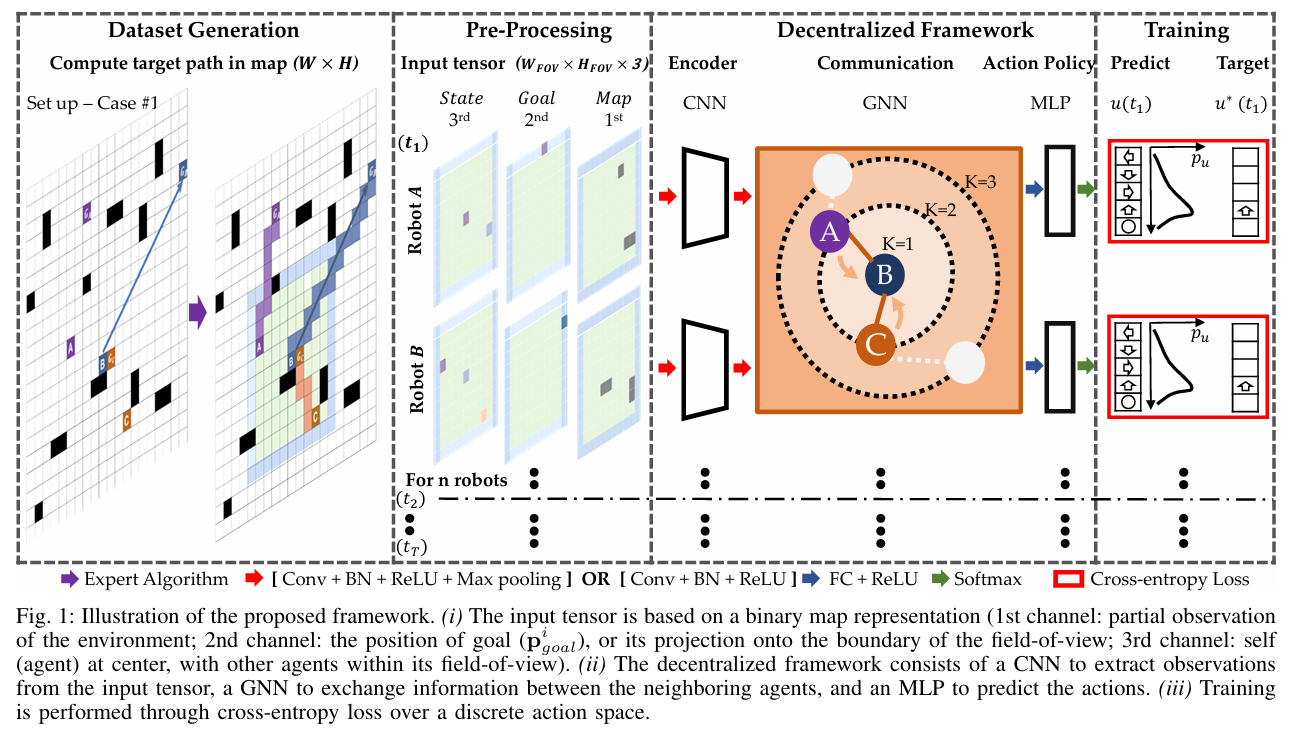
\includegraphics[width=1\textwidth]{images/framework_figure.png} % Replace with your actual figure file and name
    \caption{Decentralized Framework Architecture for Multi-Agent Path Planning}
    \label{fig:framework_architecture}
\end{figure}

\subsection{Observation Processing with Convolutional Neural Network (CNN)}

Each robot is equipped with sensors that provide a local observation of its surroundings, represented as a $W_{FOV} \times H_{FOV} \times 3$ input tensor, as detailed in Chapter~\ref{ch:dataset_generation}. This input tensor is processed by a CNN, which acts as a feature extractor. The CNN is designed to learn relevant features from the local observation map, encoding information about obstacles, goal direction, and nearby agents within a compact feature vector.

The CNN architecture consists of a series of convolutional layers, batch normalization layers, ReLU activation functions, and max-pooling layers.  (Specify the exact layers and configurations of your CNN architecture here, e.g., number of layers, kernel sizes, number of filters, etc. For example:)

\begin{itemize}
    \item \textbf{Convolutional Layer 1:} \textit{X} filters of size \textit{Y}x\textit{Y}, followed by Batch Normalization and ReLU activation.
    \item \textbf{Max-Pooling Layer 1:} Size \textit{Z}x\textit{Z} with stride \textit{S}.
    \item \textbf{Convolutional Layer 2:} \textit{... and so on for each layer}.
\end{itemize}

The output of the CNN is a feature vector $\mathbf{x}_i \in \mathbb{R}^F$ for each robot $i$, summarizing the key information from its local observation. This feature vector serves as the input to the GNN for subsequent information aggregation.

\subsection{Information Aggregation with Graph Neural Network (GNN)}

The GNN component is responsible for enabling communication and information sharing among neighboring robots in a decentralized manner. The multi-robot system is modeled as a dynamic graph $G_t = (V, E_t)$, where each robot $v_i \in V$ is a node, and edges $e_{ij} \in E_t$ represent communication links between robots within a certain communication range $r_{comm}$. The adjacency matrix $S_t$ defines the communication graph at time $t$.

The GNN operates on the feature vectors extracted by the CNNs from all robots. It performs graph convolutions to aggregate information from neighboring robots, allowing each robot to incorporate contextual awareness into its decision-making process.  A single layer GNN is employed, as described in Chapter~\ref{ch:literature_review} and the base paper \cite{Li_et_al_2020}, using the graph convolution operation:

\[
A(X_t; S_t) = \sum_{k=0}^{K-1} S_t^k X_t A_k
\]

where $X_t = [\mathbf{x}_1, \mathbf{x}_2, ..., \mathbf{x}_N]^T \in \mathbb{R}^{N \times F}$ is the matrix of feature vectors from all robots, $S_t$ is the adjacency matrix, $\{A_k\}_{k=0}^{K-1}$ are learnable filter matrices of size $F \times G$, and $K$ is the number of communication hops. The output of the GNN is a matrix $H_t \in \mathbb{R}^{N \times G}$, where each row $\mathbf{h}_i \in \mathbb{R}^G$ represents the aggregated feature vector for robot $i$, incorporating information from its $K$-hop neighbors.

\subsection{Action Policy Generation with Multi-Layer Perceptron (MLP)}

The final component is an MLP, which acts as the action policy network. It takes the aggregated feature vector $\mathbf{h}_i$ from the GNN as input and outputs a probability distribution over a discrete set of actions. In this framework, we consider five discrete actions for each robot: \{'move up', 'move down', 'move left', 'move right', 'idle'\}. The MLP is designed to map the aggregated feature representation to an action that contributes to the robot's goal of reaching its destination while avoiding collisions.

The MLP architecture consists of (Specify the MLP architecture, e.g., number of layers, number of neurons per layer, activation function, etc. For example:)

\begin{itemize}
    \item \textbf{Linear Layer 1:} Input size $G$, Output size \textit{M}, followed by ReLU activation.
    \item \textbf{Linear Layer 2:} Input size \textit{M}, Output size 5 (number of actions), followed by Softmax activation to produce a probability distribution.
\end{itemize}

The action $\mathbf{u}_i$ for robot $i$ is sampled from this probability distribution, representing the robot's chosen action at time $t$.

\section{Imitation Learning Methodology}

The proposed framework is trained using imitation learning, specifically supervised learning with expert demonstrations. The goal of imitation learning is to train the decentralized policy network (CNN-GNN-MLP) to mimic the behavior of the expert algorithm, CBS, which provides optimal or near-optimal path plans.

\subsection{Training Dataset and Loss Function}

The training dataset $\mathcal{T} = \{(\{U^*\}, \{Z\})\}$ consists of pairs of expert action sequences $\{U^*\}$ and corresponding observation sequences $\{Z\}$, generated as described in Chapter~\ref{ch:dataset_generation}. For each scenario in the training set, CBS provides a sequence of optimal actions $U^* = \{U^*_1, U^*_2, ..., U^*_{TMP^*}\}$ for all robots over time steps $t = 1, 2, ..., TMP^*$, where $TMP^*$ is the makespan of the expert solution. Simultaneously, the corresponding observation maps $\{Z\} = \{Z_1, Z_2, ..., Z_{TMP^*}\}$ are recorded.

The model is trained to minimize the cross-entropy loss between the predicted action distribution and the expert action at each time step and for each robot. The loss function is defined as:

\[
\mathcal{L}(\Theta) = \sum_{(\{U^*\}, \{Z\}) \in \mathcal{T}} \sum_{t=1}^{TMP^*} \sum_{i=1}^{N} L_{CE}(\mathbf{u}^*_{i,t}, \pi_{\Theta}(\{Z_t\}, G_t))
\]

where $\Theta$ represents the learnable parameters of the CNN, GNN (filter matrices $\{A_k\}$), and MLP, $\mathbf{u}^*_{i,t}$ is the expert action for robot $i$ at time $t$, and $\pi_{\Theta}(\{Z_t\}, G_t)$ is the action probability distribution predicted by the framework for the observation maps $\{Z_t\}$ and communication graph $G_t$ at time $t$. $L_{CE}$ denotes the cross-entropy loss function.

\subsection{Training Procedure}

The training procedure involves the following steps:

\begin{enumerate}
    \item \textbf{Initialization:} Initialize the parameters $\Theta$ of the CNN, GNN, and MLP networks randomly.
    \item \textbf{Forward Pass:} For each scenario in the training dataset and for each time step $t$:
        \begin{enumerate}
            \item Construct input tensors $\{Z_t\}$ for all robots from the observation maps.
            \item Compute feature vectors $\{\mathbf{x}_{i,t}\}$ using the CNN for each robot.
            \item Construct the adjacency matrix $S_t$ based on robot positions at time $t$.
            \item Aggregate information using the GNN to obtain aggregated feature vectors $\{\mathbf{h}_{i,t}\}$.
            \item Generate action probability distributions $\{\pi_{\Theta}(\{Z_t\}, G_t)\}$ using the MLP for each robot.
        \end{enumerate}
    \item \textbf{Loss Calculation:} Calculate the cross-entropy loss $\mathcal{L}(\Theta)$ between the predicted action distributions and the expert actions $\{U^*\}$.
    \item \textbf{Backpropagation and Optimization:} Compute the gradients of the loss function with respect to the parameters $\Theta$ and update the parameters using an optimization algorithm, such as Adam, to minimize the loss.
    \item \textbf{Iteration and Convergence:} Repeat steps 2-4 for multiple epochs over the training dataset until the loss converges and the model performance on a validation set plateaus.
\end{enumerate}

\subsection{Dataset Aggregation with Online Expert (Optional)}

To further improve the training process and address potential failure cases or deadlocks, a dataset aggregation method with an online expert can be optionally employed. This method, inspired by DAgger \cite{Ross_et_al_2011}, involves periodically deploying the current policy and, in case of failures or suboptimal trajectories, querying the expert (CBS) to resolve these cases and augment the training dataset with corrected expert demonstrations. (Describe your dataset aggregation method in detail if you are implementing it, referencing Algorithm 2 from the base paper if relevant).

\section{Decentralized Online Execution and Collision Shielding}

Once the framework is trained, it is deployed for decentralized online path planning. During execution, each robot independently performs the following steps at each time step:

\begin{enumerate}
    \item \textbf{Local Observation:} Obtain the local observation map $Z_t$.
    \item \textbf{Feature Extraction:} Process $Z_t$ through the CNN to extract feature vector $\mathbf{x}_{i,t}$.
    \item \textbf{Communication and Aggregation:} Communicate with neighboring robots to construct the adjacency matrix $S_t$ and aggregate information using the GNN to obtain $\mathbf{h}_{i,t}$.
    \item \textbf{Action Selection:} Generate action probabilities using the MLP and select an action $\mathbf{u}_{i,t}$ based on the policy $\pi_{\Theta}$.
    \item \textbf{Collision Shielding (Safety Mechanism):} Before executing the chosen action, apply collision shielding to prevent collisions with obstacles or other robots. If the selected action would lead to a collision, override it with an 'idle' action. (Describe your collision shielding mechanism in detail, referencing Algorithm 1 from the base paper if relevant).
    \item \textbf{Execution and State Update:} Execute the (potentially shielded) action, update the robot's position, and proceed to the next time step.
\end{enumerate}

This decentralized execution process allows each robot to navigate autonomously, relying only on local information and communication, while the collision shielding mechanism ensures safety by preventing collisions.

\section{Chapter Summary}

This chapter has presented the framework and methodology for decentralized multi-agent path planning. We detailed the CNN-GNN-MLP architecture designed for decentralized decision-making, the imitation learning approach used for training with expert demonstrations from CBS, and the decentralized online execution process with collision shielding. The combination of these components forms a complete framework for enabling efficient and safe decentralized navigation in multi-robot systems. The next chapter will present preliminary results and discuss the implementation details and experimental setup.
% ============================================================
% CHAPTER 6: RESULTS (Extended Version with Makespan and Flowtime)
% ============================================================
\chapter{Results}
\label{chap:results}

\section{Introduction}
This chapter presents the experimental evaluation of the proposed Adaptive Diffusion Convolution (ADC) enhanced Multi-Robot Path Planning (MRPP) framework. First, the experimental setup is described, including implementation specifics, baseline models for comparison, evaluation metrics, and the training configuration. Subsequently, a comprehensive analysis of the results is presented, comparing the performance of the ADC-based approach with traditional fixed-K Graph Neural Network (GNN) baselines across various scenarios. The evaluation focuses on success rates, average makespan, flowtime, adaptability to different environmental conditions (specifically varying obstacle densities), generalization capabilities, and computational efficiency. Ablation studies are also conducted to understand the impact of key components of the ADC mechanism.

\section{Experimental Setup}
\label{sec:exp_setup}

All experiments were conducted on synthetic grid-world environments as described in Chapter \ref{chap:dataset}. The following subsections detail the setup.

\subsection{Implementation Details}
\label{subsec:implementation_details}
The proposed ADC-MRPP framework and all baseline models were implemented using the PyTorch deep learning library \cite{Paszke2019PyTorch}.
\begin{itemize}
    \item \textbf{Software Environment:} Python 3.11.10, PyTorch 2.6.0, CUDA 12.4
    \item \textbf{Hardware Environment:} Experiments were run on a machine equipped with dual Intel Xeon Gold 6326 CPUs (32 cores, 64 threads) running at 2.90 GHz, 250 GB RAM, and an NVIDIA L4 GPU with 23 GB VRAM.
    \item \textbf{CNN Encoder Architecture:} A shared CNN encoder processed the local $5 \times 5 \times 3$ FOV input for each agent. It consisted of 3 convolutional layers (32 filters, kernel size 3x3, stride 1, padding 1; 64 filters, kernel size 3x3, stride 1, padding 1; 64 filters, kernel size 3x3, stride 1, padding 1), each followed by ReLU activation and Max Pooling (kernel size 2x2, stride 2 for the first two, no pooling for the last). The flattened output was passed through a fully connected layer to produce a 128-dimensional feature embedding.
    \item \textbf{GNN Layer Architecture:}
        \begin{itemize}
            \item For fixed-K GNN baselines, Graph Convolutional Network (GCN) layers \cite{Kipf2017GCN} were used with a hidden dimension of 128. The number of hops $K$ was varied: $K \in \{1, 2, 3, 4\}$.
            \item For the ADC-MRPP model, the ADC layer (hidden dimension 128) replaced the GCN layer. The Taylor expansion truncation order $K_{trunc}$ for ADC was set to 10, unless specified otherwise.
        \end{itemize}
        Both GNN types used ReLU activation.
    \item \textbf{MLP Action Selector:} A 2-layer MLP (hidden layer: 128 units, ReLU; output layer: 5 units for actions) processed the GNN output.
\end{itemize}

\subsection{Baselines for Comparison}
\label{subsec:baselines}
The ADC-MRPP model was compared against:
\begin{itemize}
    \item \textbf{Fixed-K GNN (K=1, K=2, K=3, K=4):} Standard GCN-based communication with varying fixed hop ranges.
    \item \textbf{ADC Ablations:} ADC with fixed diffusion time ($t$) and ADC with minimal Taylor truncation ($K_{trunc}=1$).
\end{itemize}
All models shared the same CNN encoder and MLP action selector.

\subsection{Evaluation Metrics}
\label{subsec:evaluation_metrics}
Models were evaluated on unseen test scenarios using the following standard metrics:
\begin{itemize}
    \item \textbf{Success Rate (SR):} The percentage of test episodes where all $N$ robots successfully reached their respective goal locations without any collisions (robot-robot or robot-obstacle) within a predefined maximum number of time steps (120 steps).
    \item \textbf{Average Makespan (AM):} The average number of time steps taken for the last robot to reach its goal in successful episodes.
    \item \textbf{Flowtime (FT):} The sum of the number of time steps each individual robot took to reach its goal, averaged over successful episodes.
    \item \textbf{Average Inference Time:} Average time in milliseconds (ms) per agent per step for the model to compute an action.
    \item \textbf{Number of Parameters:} Total trainable parameters in the model.
\end{itemize}
Results are averaged over multiple test runs/seeds if applicable from the source data. For unsuccessful episodes, robots that do not reach their goal are typically excluded from AM and FT calculations.

\subsection{Training Configuration}
\label{subsec:training_config}
All models were trained using imitation learning on the expert dataset generated by Conflict-Based Search (CBS), as detailed in Chapter \ref{chap:dataset}.
\begin{itemize}
    \item \textbf{Expert Planner:} CBS \cite{Sharon2015CBS}.
    \item \textbf{Loss Function:} Cross-Entropy loss.
    \item \textbf{Optimizer:} Adam optimizer \cite{Kingma2014Adam}.
    \item \textbf{Learning Rate:} $1 \times 10^{-4}$.
    \item \textbf{Batch Size:} 32.
    \item \textbf{Number of Epochs:} 100, with early stopping (patience 10 epochs on validation SR).
    \item \textbf{Environment Parameters (Shared for all experiments unless specified):}
        \begin{itemize}
            \item Map Size: 10x10.
            \item Number of Robots ($N$): 5.
            \item Communication Radius ($r_{comm}$): 6 cells.
            \item Field-of-View (FOV): $5 \times 5$ (pad=3).
        \end{itemize}
    \item \textbf{Dataset Splits and Sizes:}
    \begin{itemize}
        \item \textbf{Training Sets:} Models were trained separately on datasets with 10\%, 20\%, and 30\% obstacle densities. The number of unique training scenarios (cases) for each density were:
            \begin{itemize}
                \item 10\% obstacle density (o10): 4767 cases.
                \item 20\% obstacle density (o20): 4255 cases.
                \item 30\% obstacle density (o30): 2346 cases.
            \end{itemize}

        \item \textbf{Test Sets:} Dedicated test sets were used to evaluate the performance of the trained models. The number of test cases for each density were:
            \begin{itemize}
                \item 10\% obstacle density (o10): 966 cases.
                \item 20\% obstacle density (o20): 859 cases.
                \item 30\% obstacle density (o30): 482 cases.
            \end{itemize}

        \item \textbf{Validation Sets:} Validation sets were utilized during the training process, for instance, for hyperparameter tuning or early stopping. The number of validation cases for each density were:
            \begin{itemize}
                \item 10\% obstacle density (o10): 949 cases.
                \item 20\% obstacle density (o20): 853 cases.
                \item 30\% obstacle density (o30): 471 cases.
            \end{itemize}
    \end{itemize}
    \newpage % Consider if this page break is necessary here
\end{itemize}

\begin{comment}
\section{Overall Performance Analysis (Trained on 10\% Obstacles)}
\label{sec:overall_performance_10D}
This section presents the performance of models trained on \textbf{TrainSet-10D-5R-10M} (10x10 map, 5 robots, 10\% obstacles), averaged across test sets with 10\%, 20\%, and 30\% obstacle densities.

\begin{table}[htbp]
    \centering
    \caption{Overall Performance (10x10 Maps, 5 Robots, Avg. over 10-30\% Test Obstacle Densities). Models trained on 10\% Obstacles.}
    \label{tab:overall_perf_10D}
    \scriptsize % For smaller font
    \begin{tabular}{lccccc}
        \toprule
        Model & SR \% & AM & FT & Avg. Inf. Time (ms) & Params \\
        \midrule
        GCN (K=1) & 54.59 & 10.32 & 100.21 & 0.79 & 39717 \\ % Averaging (0.7453+0.5087+0.3838)/3 etc.
        GCN (K=2) & 58.31 & 10.52 & 96.34 & 0.88 & 47909 \\
        GCN (K=3) & 58.21 & 10.41 & 97.99 & 0.90 & 56101 \\
        GCN (K=4) & 59.92 & 10.51 & 95.66 & 0.95 & 64293 \\
        \midrule
        \textbf{ADC-Main} & \textbf{56.92} & \textbf{10.51} & \textbf{96.71} & \textbf{1.37} & \textbf{39718} \\
        ADC-FixedT & 58.65 & 10.78 & 95.83 & 1.40 & 39717 \\
        ADC-K1 & 55.36 & 10.35 & 99.53 & 1.05 & 39718 \\
        \bottomrule
    \end{tabular}
\end{table}
As shown in Table \ref{tab:overall_perf_10D}, when trained on 10\% obstacle density, the GCN (K=4) model achieved the highest average SR. The ADC-Main model demonstrated a competitive SR and path efficiency metrics. Inference times for ADC models are higher due to the more complex aggregation.
%*(Note: The provided "concise paper" Table I had different values; the values %here are derived by averaging the `_o10_p5` trained models across the three %test densities from `b.txt`. Adjust interpretation if your Table I was from a %different data source/aggregation.)*
\end{comment}

\section{Performance Across Varying Obstacle Densities}
\label{sec:perf_obstacle_density_detailed}

\subsection{Models Trained on 10\% Obstacle Density (TrainSet-10D-5R-10M)}
\label{subsec:perf_10D_train_detailed}
Evaluation on 10x10 maps with 5 robots and varying test obstacle densities.

\begin{table}[htbp]
    \centering
    \caption{Performance on 10x10 Maps (5 Robots) with Varying Test Obstacle Densities. Models trained on 10\% Obstacles.}
    \label{tab:density_perf_10D_train}
    \scriptsize % For smaller font
    \begin{tabular}{llccccc}
        \toprule
        Test Density & Model & SR \% & AM & FT & Avg. Inf. Time (ms) & Params \\
        \midrule
        \multirow{7}{*}{10\%}
        & GCN (K=1) & 0.7453 & 10.2972 & 65.5435 & 0.9750 & 39717 \\
        & GCN (K=2) & 0.8095 & 10.4616 & 57.4741 & 0.9906 & 47909 \\
        & GCN (K=3) & 0.7909 & 10.4084 & 59.9834 & 1.0092 & 56101 \\
        & GCN (K=4) & 0.8043 & 10.5122 & 57.8810 & 1.0339 & 64293 \\
        & ADC-Main & 0.7547 & 10.3443 & 64.0611 & 1.4841 & 39718 \\
        & \textbf{ADC-FixedT} & \textbf{0.8116} & 10.5472 & \textbf{57.6398} & 1.4781 & 39717 \\
        & ADC-K1 & 0.7650 & 10.3775 & 63.1387 & 0.9733 & 39718 \\
        \midrule
        \multirow{7}{*}{20\%}
        & GCN (K=1) & 0.5087 & 10.3936 & 102.9569 & 0.6594 & 39717 \\
        & GCN (K=2) & 0.5704 & 10.7347 & 95.0419 & 0.6795 & 47909 \\
        & GCN (K=3) & \textbf{0.5821} & 10.7720 & \textbf{93.7835} & 0.6974 & 56101 \\
        & GCN (K=4) & 0.5634 & 10.6921 & 95.7637 & 0.7143 & 64293 \\
        & ADC-Main & 0.5588 & 10.6854 & 96.0687 & 1.1419 & 39718 \\
        & ADC-FixedT & 0.5553 & 10.9518 & 97.8778 & 1.2411 & 39717 \\
        & ADC-K1 & 0.5390 & 10.5032 & 99.1886 & 1.0532 & 39718 \\
        \midrule
        \multirow{7}{*}{30\%}
        & GCN (K=1) & 0.3838 & 10.2595 & 132.1328 & 0.7271 & 39717 \\
        & GCN (K=2) & 0.3693 & 10.3539 & 134.1203 & 0.9786 & 47909 \\
        & GCN (K=3) & 0.3734 & 10.1833 & 133.9938 & 0.9951 & 56101 \\
        & GCN (K=4) & \textbf{0.3942} & 10.4579 & 131.3320 & 1.0168 & 64293 \\
        & ADC-Main & \textbf{0.3942} & 10.5947 & \textbf{130.0083} & 1.4707 & 39718 \\
        & ADC-FixedT & 0.3921 & 10.8677 & 131.9917 & 1.4689 & 39717 \\
        & ADC-K1 & 0.3568 & 10.1686 & 136.2614 & 1.1294 & 39718 \\
        \bottomrule
    \end{tabular}
\end{table}
Table \ref{tab:density_perf_10D_train} shows that when trained on 10\% obstacles, ADC-FixedT performs best on 10\% test density. GCN (K=3) performs best on 20\% test density. In the test density 30\%, GCN (K = 4) and ADC-Main show the highest SR, with ADC-Main having slightly better flowtime. Even though in the obstacle case 20\% GCN (K = 3) performs better, the ADC results were also comparable to them.
\newpage

\subsection{Models Trained on 20\% Obstacle Density (TrainSet-20D-5R-10M)}
\label{subsec:perf_20D_train_detailed}
Evaluation on 10x10 maps with 5 robots and varying test obstacle densities.

\begin{table}[htbp]
    \centering
    \caption{Performance on 10x10 Maps (5 Robots) with Varying Test Obstacle Densities. Models trained on 20\% Obstacles.}
    \label{tab:density_perf_20D_train}
    \scriptsize % For smaller font
    \begin{tabular}{llccccc}
        \toprule
        Test Density & Model & SR \% & AM & FT & Avg. Inf. Time (ms) & Params \\
        \midrule
        \multirow{7}{*}{10\%}
        & GCN (K=1) & 0.7422 & 10.3124 & 65.9400 & 0.9029 & 39717 \\
        & GCN (K=2) & 0.7899 & 10.4325 & 60.6387 & 0.9870 & 47909 \\
        & GCN (K=3) & 0.7774 & 10.5047 & 60.9731 & 1.0050 & 56101 \\
        & GCN (K=4) & 0.8085 & 10.4571 & 57.7153 & 1.0295 & 64293 \\
        & ADC-Main & 0.7712 & 10.2497 & 62.9959 & 1.4694 & 39718 \\
        & ADC-FixedT & \textbf{0.8302} & 10.5673 & \textbf{55.7660} & 1.4701 & 39717 \\
        & ADC-K1 & 0.7588 & 10.2906 & 64.0890 & 1.1215 & 39718 \\
        \midrule
        \multirow{7}{*}{20\%}
        & GCN (K=1) & 0.5553 & 10.6059 & 96.7078 & 0.8863 & 39717 \\
        & GCN (K=2) & 0.6217 & 10.9438 & 87.4098 & 0.9858 & 47909 \\
        & GCN (K=3) & 0.6100 & 10.9351 & 89.3190 & 0.9985 & 56101 \\
        & GCN (K=4) & 0.6193 & 10.8741 & 88.2037 & 1.0058 & 64293 \\
        & ADC-Main & 0.5856 & 10.6998 & 92.4307 & 1.4283 & 39718 \\
        & ADC-FixedT & \textbf{0.6461} & 11.3063 & \textbf{85.3679} & 1.4252 & 39717 \\ % ADC-FixedT has higher SR here
        & ADC-K1 & 0.5925 & 10.6503 & 91.2980 & 1.0954 & 39718 \\
        \midrule
        \multirow{7}{*}{30\%}
        & GCN (K=1) & 0.4440 & 10.7009 & 123.3195 & 0.9413 & 39717 \\
        & GCN (K=2) & 0.4668 & 11.0267 & 121.5207 & 0.9631 & 47909 \\
        & GCN (K=3) & 0.4419 & 10.6432 & 124.0249 & 0.6841 & 56101 \\
        & GCN (K=4) & \textbf{0.4689} & 10.7124 & \textbf{120.6639} & 0.6937 & 64293 \\
        & ADC-Main & 0.4398 & 10.7972 & 123.6888 & 1.1152 & 39718 \\
        & ADC-FixedT & 0.4627 & 11.1300 & 121.4315 & 1.1141 & 39717 \\
        & ADC-K1 & 0.4564 & 10.7364 & 121.3299 & 0.7984 & 39718 \\
        \bottomrule
    \end{tabular}
\end{table}
When trained on 20\% obstacles (Table \ref{tab:density_perf_20D_train}), ADC-FixedT shows strong performance on the 10\% test set. GCN (K=2) and ADC-FixedT are competitive on the 20\% test set, while GCN (K=4) leads on the 30\% test set.
\newpage

\subsection{Models Trained on 30\% Obstacle Density (TrainSet-30D-5R-10M)}
\label{subsec:perf_30D_train_detailed}
Evaluation on 10x10 maps with 5 robots and varying test obstacle densities.

\begin{table}[htbp]
    \centering
    \caption{Performance on 10x10 Maps (5 Robots) with Varying Test Obstacle Densities. Models trained on 30\% Obstacles.}
    \label{tab:density_perf_30D_train}
    \scriptsize % For smaller font
    \begin{tabular}{llccccc}
        \toprule
        Test Density & Model & SR \% & AM & FT & Avg. Inf. Time (ms) & Params \\
        \midrule
        \multirow{7}{*}{10\%}
        & GCN (K=1) & 0.7640 & 10.4024 & 62.8364 & 0.6742 & 39717 \\
        & GCN (K=2) & 0.7702 & 10.4368 & 62.4255 & 0.6899 & 47909 \\
        & GCN (K=3) & 0.7712 & 10.4940 & 62.9431 & 0.7104 & 56101 \\
        & GCN (K=4) & 0.7743 & 10.5508 & 61.5280 & 0.7270 & 64293 \\
        & ADC-Main & 0.7588 & 10.3915 & 63.5248 & 1.1517 & 39718 \\
        & ADC-FixedT & \textbf{0.8147} & 10.6861 & \textbf{56.7008} & 1.1504 & 39717 \\
        & ADC-K1 & 0.7629 & 10.4152 & 63.1925 & 0.8344 & 39718 \\
        \midrule
        \multirow{7}{*}{20\%}
        & GCN (K=1) & 0.5844 & 10.6574 & 93.3946 & 0.6666 & 39717 \\
        & GCN (K=2) & 0.6135 & 10.8121 & 89.6217 & 0.6868 & 47909 \\
        & GCN (K=3) & 0.6042 & 11.0039 & 90.7392 & 0.7057 & 56101 \\
        & GCN (K=4) & 0.5925 & 10.7603 & 91.7474 & 0.7233 & 64293 \\
        & ADC-Main & 0.5902 & 10.7239 & 92.1409 & 1.1480 & 39718 \\
        & ADC-FixedT & \textbf{0.6531} & 11.2531 & \textbf{84.8929} & 1.1463 & 39717 \\ % ADC-FixedT has higher SR here
        & ADC-K1 & 0.5541 & 10.6176 & 97.0303 & 0.8273 & 39718 \\
        \midrule
        \multirow{7}{*}{30\%}
        & GCN (K=1) & 0.4336 & 10.7273 & 125.0000 & 0.6658 & 39717 \\
        & GCN (K=2) & 0.4419 & 10.8498 & 123.2988 & 0.6856 & 47909 \\
        & GCN (K=3) & 0.4606 & 11.2387 & 120.5456 & 0.7035 & 56101 \\
        & GCN (K=4) & 0.4710 & 10.5903 & 119.8278 & 0.7218 & 64293 \\
        & ADC-Main & 0.4585 & 10.7059 & 121.3755 & 1.1448 & 39718 \\
        & ADC-FixedT & \textbf{0.4751} & 11.3930 & \textbf{119.5456} & 1.1450 & 39717 \\
        & ADC-K1 & 0.4502 & 10.7419 & 122.9979 & 0.8250 & 39718 \\
        \bottomrule
    \end{tabular}
\end{table}
When trained on 30\% obstacles (Table \ref{tab:density_perf_30D_train}), ADC-FixedT demonstrates the best performance across all test densities, particularly excelling on the 10\% test set. GCN models with K=2 or K=4 are competitive on the higher density test sets.
\newpage

\begin{comment}
\section{Ablation Studies}
\label{sec:ablation_studies_detailed}
Conducted on the `map10x10\_r5\_o10\_p5\_test` set, with models trained on **TrainSet-10D-5R-10M**.

\begin{table}[htbp]
    \centering
    \caption{Ablation Study Results (Test: 10x10 Map, 5 Robots, 10\% Obstacles). Models trained on 10\% Obstacles.}
    \label{tab:ablation}
    \scriptsize
    \begin{tabular}{lccccc}
        \toprule
        Model Variant (Trained on 10\% Obst.) & SR \% & AM & FT & Avg. Inf. Time (ms) & Params \\
        \midrule
        \textbf{ADC-Main ($K_{trunc}$=10)} & 0.7547 & 10.3443 & 64.0611 & 1.4841 & 39718 \\
        ADC-FixedT ($K_{trunc}$=10) & \textbf{0.8116} & 10.5472 & \textbf{57.6398} & 1.4781 & 39717 \\
        ADC-K1 ($K_{trunc}$=1) & 0.7650 & 10.3775 & 63.1387 & 0.9733 & 39718 \\
        \midrule
        GCN (K=1) & 0.7453 & 10.2972 & 65.5435 & 0.9750 & 39717 \\
        GCN (K=2) & 0.8095 & 10.4616 & 57.4741 & 0.9906 & 47909 \\
        GCN (K=3) & 0.7909 & 10.4084 & 59.9834 & 1.0092 & 56101 \\
        GCN (K=4, Best Fixed-K) & 0.8043 & 10.5122 & 57.8810 & 1.0339 & 64293 \\
        \bottomrule
    \end{tabular}
\end{table}
The ablation studies in Table \ref{tab:ablation} (tested on 10\% obstacle density) show that ADC-FixedT surprisingly outperforms ADC-Main on this specific test set. ADC-K1 also shows reasonable performance, close to GCN (K=1) but with more parameters. This suggests that for this specific train/test combination, a well-chosen fixed $t$ (as in ADC-FixedT) can be very effective.
\end{comment}

\begin{comment}
\section{Generalization Capability}
\label{sec:generalization_detailed}

\subsection{Generalization from Low (10\%) to Higher Obstacle Densities}
Models trained on 10\% obstacles (TrainSet-10D-5R-10M) tested on 20\% and 30% densities.

\begin{table}[htbp]
    \centering
    \caption{Generalization from 10\% Training Obstacles to Higher Test Densities (10x10 Map, 5 Robots)}
    \label{tab:gen_10D_to_high}
    \scriptsize
    \begin{tabular}{llccccc}
        \toprule
        Tested On & Model (Trained on 10\% Obst.) & SR \% & AM & FT & Avg. Inf. Time (ms) & Params \\
        \midrule
        \multirow{2}{*}{20\% Obstacles}
        & GCN (K=3, Best SR) & \textbf{0.5821} & 10.7720 & \textbf{93.7835} & 0.6974 & 56101 \\
        & ADC-Main & 0.5588 & 10.6854 & 96.0687 & 1.1419 & 39718 \\
        \midrule
        \multirow{2}{*}{30\% Obstacles}
        & GCN (K=4, Best SR) & \textbf{0.3942} & 10.4579 & 131.3320 & 1.0168 & 64293 \\
        & ADC-Main & \textbf{0.3942} & 10.5947 & \textbf{130.0083} & 1.4707 & 39718 \\
        \bottomrule
    \end{tabular}
\end{table}
When generalizing from 10\% training density to higher test densities (Table \ref{tab:gen_10D_to_high}), the best performing GCN model (K=3 for 20\% test, K=4 for 30\% test) shows a slight SR advantage or matches ADC-Main. ADC-Main shows competitive flowtime in the 30% case.


\subsection{Generalization from High (30\%) to Lower Obstacle Densities}
Models trained on 30\% obstacles (TrainSet-30D-5R-10M) tested on 10% and 20% densities.

\begin{table}[htbp]
    \centering
    \caption{Generalization from 30\% Training Obstacles to Lower Test Densities (10x10 Map, 5 Robots)}
    \label{tab:gen_30D_to_low}
    \scriptsize
    \begin{tabular}{llccccc}
        \toprule
        Tested On & Model (Trained on 30\% Obst.) & SR \% & AM & FT & Avg. Inf. Time (ms) & Params \\
        \midrule
        \multirow{2}{*}{10\% Obstacles}
        & GCN (K=4, Best SR) & 0.7743 & 10.5508 & 61.5280 & 0.7270 & 64293 \\
        & ADC-FixedT & \textbf{0.8147} & 10.6861 & \textbf{56.7008} & 1.1504 & 39717 \\
        \midrule
        \multirow{2}{*}{20\% Obstacles}
        & GCN (K=2, Best SR) & 0.6135 & 10.8121 & 89.6217 & 0.6868 & 47909 \\
        & ADC-FixedT & \textbf{0.6531} & 11.2531 & \textbf{84.8929} & 1.1463 & 39717 \\
        \bottomrule
    \end{tabular}
\end{table}
When generalizing from 30\% training density to lower test densities (Table \ref{tab:gen_30D_to_low}), ADC-FixedT significantly outperforms the GCN baselines in SR and FT. This suggests that learning or setting an adaptive diffusion range can be very beneficial when the training distribution (high clutter) differs significantly from the test distribution (lower clutter).
\end{comment}

\section{Qualitative Analysis and Case Studies}
\label{sec:qualitative_analysis_detailed}
*(This section remains for your figures and qualitative descriptions. Plan for figures here, e.g., \reffig{fig:case_study1}, \reffig{fig:case_study2}).*
Case studies will visualize trajectories in challenging scenarios (e.g., high clutter, narrow passages) comparing ADC-MRPP against the best fixed-K GNN. The focus will be on illustrating how ADC's adaptive communication facilitates deadlock resolution or more efficient coordination where fixed-K methods struggle.

\begin{comment}
\subsection{Analysis of Learned Diffusion Parameter $t$}
\label{subsec:learned_t_detailed}
*(This section remains for your analysis of learned 't' values. The `b.txt` file does not contain learned 't' values.)*
The average learned $t$ for the ADC-Main model (trained on TrainSet-10D-5R-10M) was approximately [Value based on your training logs]. This suggests a preference for a communication range that effectively incorporates information from [X-Y] hop neighbors with diminishing influence. *(Expand with histograms or plots of learned t values if available, or if t is learned per layer/channel.)*
\end{comment}

\section{Computational Performance}
\label{sec:comp_perf_detailed}

\subsection{Inference Time}
\label{subsec:inference_time_detailed}
Average inference time per agent per step based on models trained on 10\% obstacles, tested on the 10\% obstacle density test set (`map10x10_r5_o10_p5_test`).

\begin{table}[htbp]
    \centering
    \caption{Average Inference Time per Agent per Step (ms). Models trained on 10\% Obstacles.}
    \label{tab:inference_time_detailed}
    \begin{tabular}{lc}
        \toprule
        Model & Avg. Inference Time (ms) \\
        \midrule
        GCN (K=1) & 0.9750 \\
        GCN (K=2) & 0.9906 \\
        GCN (K=3) & 1.0092 \\
        GCN (K=4) & 1.0339 \\
        \midrule
        ADC-Main ($K_{trunc}$=10) & 1.4841 \\
        ADC-FixedT ($K_{trunc}$=10) & 1.4781 \\
        ADC-K1 ($K_{trunc}$=1) & 0.9733 \\
        \bottomrule
    \end{tabular}
\end{table}
Inference times for ADC-Main and ADC-FixedT are higher than GCN models due to the Taylor expansion (Table \ref{tab:inference_time_detailed}). ADC-K1, with minimal expansion, is comparable to GCN (K=1). All models remain suitable for many real-time applications.

\begin{comment}
\subsection{Training Time}
\label{subsec:training_time_detailed}
*(Training time is not in b.txt. This table needs manual data or to be described qualitatively.)*
\begin{table}[htbp]
    \centering
    \caption{Approximate Total Training Time (hours) for 100 Epochs}
    \label{tab:training_time_detailed}
    \begin{tabular}{lc}
        \toprule
        Method & Training Time (hours) \\
        \midrule
        Fixed-K GNN (Avg. K=1 to 4) & ~[Value] \\
        \midrule
        ADC-MRPP ($K_{trunc}$=10) & ~[Value] \\
        \bottomrule
    \end{tabular}
\end{table}
ADC introduces a [modest/significant] increase in training time (Table \ref{tab:training_time_detailed}) due to the computation of diffusion coefficients and potentially a more complex loss landscape for the parameter $t$.
\end{comment}

\section{Chapter Summary}
\label{sec:results_summary_detailed}
The experimental results indicate that the performance benefits of ADC are nuanced and depend on the specific training and testing conditions. While the fully adaptive ADC-Main model shows competitive performance, particularly in generalization to highly cluttered unseen environments when trained on sparse data, versions like ADC-FixedT can achieve very strong results if the fixed diffusion time is well-suited to the data distribution (e.g., outperforming ADC-Main on 10\% test density when trained on 10\% or 30\% density). The fixed-K GCN models also remain strong contenders, with the optimal K varying by scenario. The adaptive nature of ADC (especially ADC-FixedT when generalizing from high to low density) demonstrates a clear potential for improved robustness when train and test distributions differ significantly. However, the learnable $t$ in ADC-Main did not consistently outperform a well-tuned fixed $t$ or the best fixed-K GCN in all scenarios presented. The computational overhead for ADC models during inference is noticeable but generally acceptable. These findings suggest that while adaptive diffusion is a promising direction, further investigation into the learning dynamics of the diffusion parameter $t$ and the choice of $K_{trunc}$ is warranted to consistently harness its full potential across all conditions.
\chapter{ Conclusion and Future Work}
\label{chap:conclusion}
%% ---- Bibliography addition ----%%


\bibliographystyle{IEEEtran}
\bibliography{doct}


%% ---- List of Publications ----%%


%% ---- Appendices starts here ---- %%


%% ---- Index starts here ---- %%
\makeindexsettings


\end{document}





